\begin{tcolorbox}[colback=green!5!white, colframe=green!75!black]
\textit{Esta relación no suele caer en el examen, la 2 y la 3 sí.}
\end{tcolorbox}

\textbf{Podemos ver los códigos de los ejercicios 1,3,4 en el apartado de Asignaturas/Tercer Año/IA/Teoria/Capitulos/Elementos\_Relacion\_1 en la web del blog de ismael.}

\subsection*{Ejercicio 1}

Una hormiga artificial vive en un mundo bidimensional cuadriculado y desarrolla un 
comportamiento  que  le  permite  seguir  un  rastro  de  feromonas  a  lo  largo  de  un  conjunto  de 
casillas  previamente  marcadas  (el  tamaño  del  rastro  es  de  una  casilla).  La  hormiga  ocupa  una 
sola casilla y puede encarar las casillas que se encuentran arriba, a la derecha, a la izquierda y 
debajo  de  la  posición  en  la  que  se  encuentra.  La  hormiga  puede  llevar  a  cabo  tres  acciones: 
moverse a una celda hacia adelante (actFORWARD), girar a la izquierda permaneciendo en la 
misma casilla (actTURN\_L) y girar a la derecha permaneciendo en la misma casilla 
(actTURN\_R).  La  hormiga  puede  percibir  si  la  casilla  que  tiene  delante  (en  el  sentido  del 
movimiento) tiene feromona.

\begin{enumerate}
    \item Especificar  un  sistema  de  reglas  para  controlar  el  comportamiento  de  la  hormiga  en  el 
    seguimiento del rastro de la feromona. Suponer inicialmente a la hormiga en una casilla en 
    la que puede percibir el rastro de feromona.
    \item Resuelva el problema anterior con la siguiente restricción: la hormiga, una vez que llega a 
    una nueva casilla, no puede girar más de 180 grados desde la posición inicial.
\end{enumerate}

\subsubsection*{Solución}
Debemos de tener en cuenta las características de los agentes reactivos:
\begin{itemize}
    \item Sensores:
    \begin{itemize}
        \item Feromona: booleano.
    \end{itemize}
    \item Acciones.
    \begin{itemize}
        \item actFORWARD.
        \item actTURN\_L.
        \item actTURN\_R.
    \end{itemize}
    \item Reglas.
    \begin{itemize}
        \item Si percibo feronomonas delante de mi $\rightarrow$ actFORWARD y he\_girado\_Derecha = false.
        \item Si no feromona y no he\_girado\_Derecha $\rightarrow$ actTURN\_R y he\_girado\_Derecha = true.
        \item Si no feromona y he\_girado\_Derecha $\rightarrow$ actTURN\_L.
        % \item Si no (else) percibo feronomonas delante de mi, actTURN\_L o actTURN\_R (dependiento del que sea más conveniente).
    \end{itemize}
    \item Variables de estado.
    \begin{itemize}
        \item He\_girado\_Derecha (booleano). Se debe de inicializar a falso.
    \end{itemize}
\end{itemize}

Con esto tenemos definido completamente nuestro agente.

\subsubsection*{Anotaciones sobre el desarrollo del ejercicio}
\begin{itemize}
    \item Vemos que nuestra solución tiene fallos debido a que siempre esta girando hacia la derecha, así que debemos de hacer uso de las variables de estado para solucionar este problema.
    \item Tenemos el problema de que si se cruzan los caminos no pasará por uno de ellos.
\end{itemize}


\subsection*{Ejercicio 2}

La avispa hembra del género Sphex, deja sus huevos dentro de un grillo que ha paralizado y ha 
llevado  a  su  nido.  Las  larvas  de  la  avispa  salen  del  grillo  y  se  alimentan  de  él.  La  avispa 
presenta el siguiente comportamiento: lleva el grillo paralizado a su nido, lo deja en el umbral 
del nido, entra dentro del nido para ver si todo está correcto, sale, y entonces arrastra al grillo 
hacia  su  interior.  Si  el  grillo  se  mueve  cuando  la  avispa  está  en  el  interior  haciendo  la 
inspección preliminar, la avispa saldrá del nido, volverá a colocar el grillo en el umbral, pero no 
dentro, y repetirá el procedimiento de entrar en el nido para ver si todo está correcto. Si el grillo 
se mueve otra vez mientras la avispa está dentro del nido, ésta volverá a salir y colocar el grillo 
en  el  umbral,  entrando  de  nuevo  en  el  nido  para  realizar  la  inspección  preliminar.  En  una 
ocasión,  este  procedimiento  se  repitió  cuarenta  veces.  Define  características  y  acciones  para 
diseñar un agente reactivo que se corresponda con el comportamiento de la avispa.

\subsubsection*{Solución}

\begin{itemize}
    \item Sensores.
    \begin{itemize}
        \item Grillo\_movido: booleano.
    \end{itemize}
    \item Acciones.
    \begin{itemize}
        \item actLlevar\_Nido.
        \item actDejar\_Umbral.
        \item actEntrar\_Nido.
        \item actSalir\_Nido.
    \end{itemize}
    \item Reglas.
    \begin{itemize}
        \item Si grillo\_movido, actDejar\_Umbral.
        \item Si no grillo\_movido, actEntrar\_Nido.
    \end{itemize}
    \item Variables de estado.
    \begin{itemize}
        \item Grillo\_movido: booleano. Se debe de inicializar a falso.
    \end{itemize}
\end{itemize}   

\subsection*{Ejercicio 3}

Supongamos  que  un  agente  trabaja  sobre  un  tablero  formado  por  NxN  casillas.  Sobre  este 
tablero se definen dos zonas: una "zona interior" formada por un tablero de (N-2)x(N-2) casillas 
inscrito  en  el  tablero  general,  y  una  "zona  exterior"  formada  por  el  resto  de  las  casillas. Separando ambas zonas aparece una línea gruesa negra denominada "Frontera". En la figura se 
muestra un ejemplo de la configuración de un tablero 7x7. 
El  cometido  del  robot  consiste  en  llevar  todos  los  obstáculos  que  se  encuentren  en  la  zona 
interior a la zona exterior. El robot siempre se debe encontrar en la 
zona interior, y no debe nunca traspasar la frontera. 
Para  realizar  esta  tarea,  el  robot  dispone  de  3  sensores,  un  sensor 
de  choque  "BUMPER"  que  le  permite  detectar  el  obstáculo,  un 
sensor de infrarrojos "CNY70" que permite ver dónde está la línea 
de  la  Frontera,  y  una  brújula  digital  "Brujula"  que  le  indica  su 
orientación en el avance. Los dos primeros sensores se encuentran 
situados  en  la  parte  frontal  del  robot.  La  brújula  sólo  devuelve  4 
valores: 0, 1, 2 y 3, representando respectivamente Norte, Este, Sur 
y Oeste. 
 
Las acciones que puede realizar el robot son las siguientes: 
\begin{enumerate}
    \item Avanzar: Avanza una casilla en la dirección que marca su brújula siempre que no tenga 
    un obstáculo delante. 
    \item Retroceder:  Retrocede  una  casilla  en  la  dirección  contraria  a  la  que  indica  su  brújula, 
    siempre que no tenga un obstáculo detrás. 
    \item GirarI: Gira sin moverse de la casilla hacía la izquierda. 
    \item GirarD: Gira sin moverse de la casilla hacía la derecha. 
    \item Nada: No realiza ninguna acción 
    \item Empujar: Avanza una casilla en la dirección que marca su brújula. Para que está acción 
    tenga efecto, debe estar activado el sensor de choque. 
\end{enumerate}

Se pide: 
\begin{itemize}
    \item[a)] Definir  las  variables  de  estado  (nombre  e  descripción)  y  las  reglas  de  producción 
    necesarias  para  diseñar  un  agente  reactivo  con  memoria  que  partiendo  de  una  casilla 
    desconocida dentro de la zona interior de un tablero de dimensiones también 
    desconocidas (nunca superiores a 99x99), sea capaz de calcular la dimensión de la zona 
    interior, suponiendo que en el tablero no hay obstáculos. 
    \item [b)] Definir  las  variables  de  estado  y  las  reglas  de  producción  necesarias  que  permitan  al 
    robot localizar el obstáculo en el tablero. 
    \item [c)] Suponiendo  que  el  robot  se  encuentra  orientado  hacía  el  obstáculo  en  una  casilla 
    adyacente (es decir, el sensor BUMPER está activado) y que el obstáculo se encuentra 
    en  una  casilla  interna  del  tablero  que  no  es  adyacente  con  ninguna  casilla  pegada  a  la 
    frontera,  definir  las  variables  de  estado  y  las  reglas  de  producción  necesarias  que 
    permitan  al  robot  expulsar  el  obstáculo  hacía  la  zona  exterior,  arrastrándolo  por  el 
    camino más corto de casillas. 
\end{itemize}

\begin{figure}[H]
    \centering
    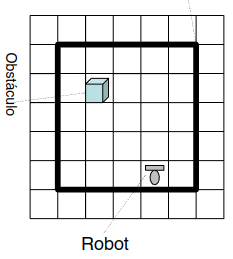
\includegraphics[width=0.35\textwidth]{images/ej3rel1.png}
    \caption{Imagen del tablero.}
    \label{fig:tablero}
\end{figure}

% \begin{figure}[h]
%     \centering
%     \begin{tikzpicture}
%         % Cuadrícula
%         \draw[step=0.5cm,gray,very thin] (0,0) grid (2.5,2.5);
        
%         % Borde del área negra
%         \draw[very thick] (0.5,0.5) rectangle (2,2);
        
%         % Obstáculo
%         \filldraw[gray!30] (1,1.75) rectangle (1.25,2);
%         \draw (1,1.75) rectangle (1.25,2);
        
%         % Robot
%         \filldraw[gray!30] (1.75,0.75) circle (0.2);
%         \draw (1.75,0.8) -- (1.75,0.65);
%         \draw (1.65,0.5) -- (1.85,0.5);
        
%         % Etiquetas
%         \node[rotate=90] at (-0.3,1.25) {Obstáculo};
%         \node at (1.25,-0.3) {Robot};
%     \end{tikzpicture}
%     \caption{Tablero con tikz.}
% \end{figure}


\subsubsection*{Solución a)}

\begin{itemize}
    \item Sensores.
    \begin{itemize}
        \item BUMPER: booleano.
        \item CNY70: booleano.
        \item Brujula: entero (0,1,2,3).
    \end{itemize}
    \item Acciones.
    \begin{itemize}
        \item Avanzar.
        \item Retroceder.
        \item GirarI.
        \item GirarD.
        \item Nada.
        \item Empujar.
    \end{itemize}
    \item Variables de estado.
    \begin{itemize}
        \item estoy\_contando: booleano. Se debe de inicializar a falso.
        \item estoy\_girando: booleano. Se debe de inicializar a falso.
        \item contador: entero. Se debe de inicializar a 0.
    \end{itemize}
    \item Reglas.
    \begin{itemize}
        \item Si no estoy\_contando y no estoy\_girando y no CNY70 $\rightarrow$ avanzar.
        \item Si no estoy\_contando y no estoy\_girando y CNY70 $\rightarrow$ girarI y estoy\_girando = true.
        \item Si estoy\_girando $\rightarrow$ girarI, estoy\_contado = true, contador++, estoy\_girando = false.
        \item Si estoy\_contando y no estoy\_girando y no CNY70 $\rightarrow$ avanzar, contador++.
        \item Si estoy\_contando y no estoy\_girando y CNY70 $\rightarrow$ Terminaríamos, podemos devolver el \underline{IDLE} y el \underline{contador}.
        \end{itemize}
\end{itemize}

\subsubsection*{Solución b)}

\begin{itemize}
    \item En este punto cambiamos la variables de estado: \begin{itemize}
        \item $\text{fase\_giro}(0,1,2) = [0] \text{ inicialmente 0}$
        \item girar\_izq: booleano = true (inicialmente)
    \end{itemize}
    \item Reglas.
    \begin{itemize}
        \item Si BUMPER $\rightarrow$ \underline{IDLE}
        \item Si no CNY70 y fase\_giro == 0 $\rightarrow$ Avanzar
        \item SI CNY70 y y fase\_giro == 0 y girar\_izq $\rightarrow$ GirarI y fase\_giro = 1
        \item Si no CNY70 y fase\_giro == 1 $\rightarrow$ Avanzar y fase\_giro == 2
        \item Si fase\_giro == 2 y girar\_izq $\rightarrow$ GirarI, fase\_giro=0 y girar\_izq = false 
        \item SI CNY70 y fase\_giro == 0 y no girar\_izq $\rightarrow$ GirarD y fase\_giro = 1
        \item Si fase\_giro == 2 y no girar\_izq $\rightarrow$ GirarD, fase\_giro==0 y girar\_izq = true
        \item Si CNY70 y fase\_giro == 1 y no giro\_izq $\rightarrow$ GirarD y fase\_giro=0
        \item Si CNY70 y fase\_giro == 1 y gira\_izq $\rightarrow$ GirarI y fase\_giro=0
    \end{itemize}
\end{itemize}

%\subsubsection*{Solución c)}





\subsection*{Ejercicio 4}

Supongamos que tenemos un robot sobre un mapa bidimensional discreto de tamaño NxM. El 
robot puede realizar las acciones de Avanzar y Girar en el sentido de las agujas del reloj. El 
robot posee un sistema de posicionamiento sobre el mapa que le devuelve sus coordenadas 
absolutas “(robotX, robotY)” dentro del mapa. 

Suponiendo que en el mapa hay obstáculos fijos (paredes), y que el robot se encuentra ubicado 
dentro de ese mapa en una posición concreta, definir un comportamiento reactivo para el mismo 
que le permita desplazarse hasta una coordenada objetivo “(ObjX, ObjY)”. Para ello, definir las 
variables de estado necesarias y el sistema de reglas de producción que reproducen el 
comportamiento requerido.

%\subsubsection*{Solución}



\subsection*{Ejercicio 5}

Idear una función de potencial artificial (con componentes repulsivos y atractivos) que pueda 
ser utilizada para guiar un robot desde cualquier casilla del mundo bidimensional cuadriculado 
de la figura siguiente, a la casilla objetivo que está marcada con una X (suponer que las posibles 
acciones que puede ejecutar el robot son ir al norte, sur, este y oeste). ¿Tienen las componentes 
repulsivas y atractivas algún mínimo local? Si es así, ¿dónde?

\begin{figure}[H]
    \centering
    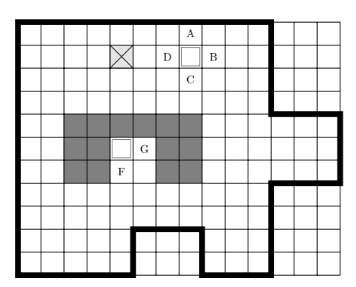
\includegraphics[width=0.5\textwidth]{images/ej5rel1.png}
    \caption{Imagen del mundo bidimensional cuadriculado.}
    \label{fig:mundo}
\end{figure}

\subsubsection*{Solución}

Cálculo de una casilla física (Potencial artificial): 

\begin{itemize}
    \item Componente atractica:
    $p_a(X) = K_1d(X)^2$
    \item Componente repulsica: 
    $p_r(X) = \frac{k_2}{d_0(X)^2}$
\end{itemize}

Aplicando las fórmulas en el ejercicio:

\begin{align*}
    P_a(x) = d(x,obj)^2 \\
    P_r(x) = \frac{1}{d(x,obst)^2} \\
    P(x) = P_a(x)+P_r(x) \\
    P(A) = 4^2 +  \frac{1}{1^2} = 17\\
    P(B) = 4^2 + \frac{1}{2^2} = 16,25\\
    P(C) = 4^2 + \frac{1}{2^2} = 16,25\\
    P(D) = 2^2 + \frac{2^2}{2^2} = 4,25
\end{align*}

Como solución, si debemos de elegir uno en base al potencial nos quedaríamos con D.

Para el 2º apartado:

\begin{align*}
    P(G) = 5^2+ \frac{1}{1^2} = 26 \\
    P(F) = 5^2+ \frac{1}{1^2} = 26
\end{align*}

En este caso al haber empate da igual cual cogemos.

\begin{align}
    P(\text{casilla marcada}) = 4^2 + \frac{1}{1^2} = 17
\end{align}

La casilla del cuadrado es la que menos potencial tiene por lo que debemos de quedarnos con esa (Ecuación 1.1).

